\documentclass[]{article}
\usepackage{geometry}
\geometry{
a4paper,
total={170mm,257mm},
left=20mm,
top=20mm,
}
\usepackage{booktabs} 
\usepackage{longtable}
\usepackage{appendix}
\usepackage{graphicx}
\usepackage{subcaption}
\usepackage{listings}
\usepackage[justification=centering]{caption}
\usepackage{hyperref}
\usepackage{enumitem}
\usepackage[utf8]{inputenc}
\usepackage{float}
\usepackage[autostyle]{csquotes} 
\DeclareTextFontCommand{\helvetica}{\fontfamily{phv}\selectfont}
\setlength{\parindent}{4em}
\setlength{\parskip}{1em}
\linespread{1.5}

\usepackage[table]{xcolor}
\usepackage{graphicx}
\usepackage{adjustbox}

\title{Memòria del treball de final de màster}
\date{20 de Maig 2019}
\author{Vasyl Druchkiv \\ Estudiant del Màster de Bioestadística i Bioinformàtica}
\renewcommand{\contentsname}{Índice}
\usepackage{setspace}


\renewcommand\paragraph{\@startsection{paragraph}{4}{\z@}%
{-2.5ex\@plus -1ex \@minus -.25ex}%
{1.25ex \@plus .25ex}%
{\normalfont\normalsize\bfseries}}

\begin{document}
\maketitle
\makeatletter

\makeatother
\begin{spacing}{0.1}
\tableofcontents
\end{spacing}

\begin{center}
\noindent\rule{8cm}{0.4pt}
\end{center}

\section{Introducció}

\begin{figure}[H]
\centering
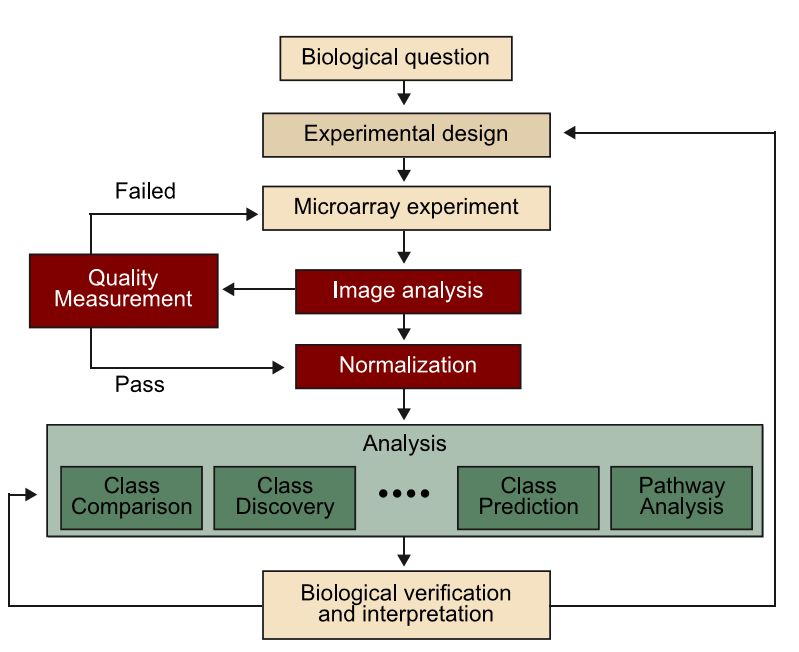
\includegraphics[width=0.9\textwidth]{Pipeline_Microarray.jpg} 
\caption{El procès d'anàlisi de microarrays}
\end{figure}


\section{Anàlisi de les rutes - final del pipeline d'anàlisi d'expressió}


\begin{figure}[H]
\centering
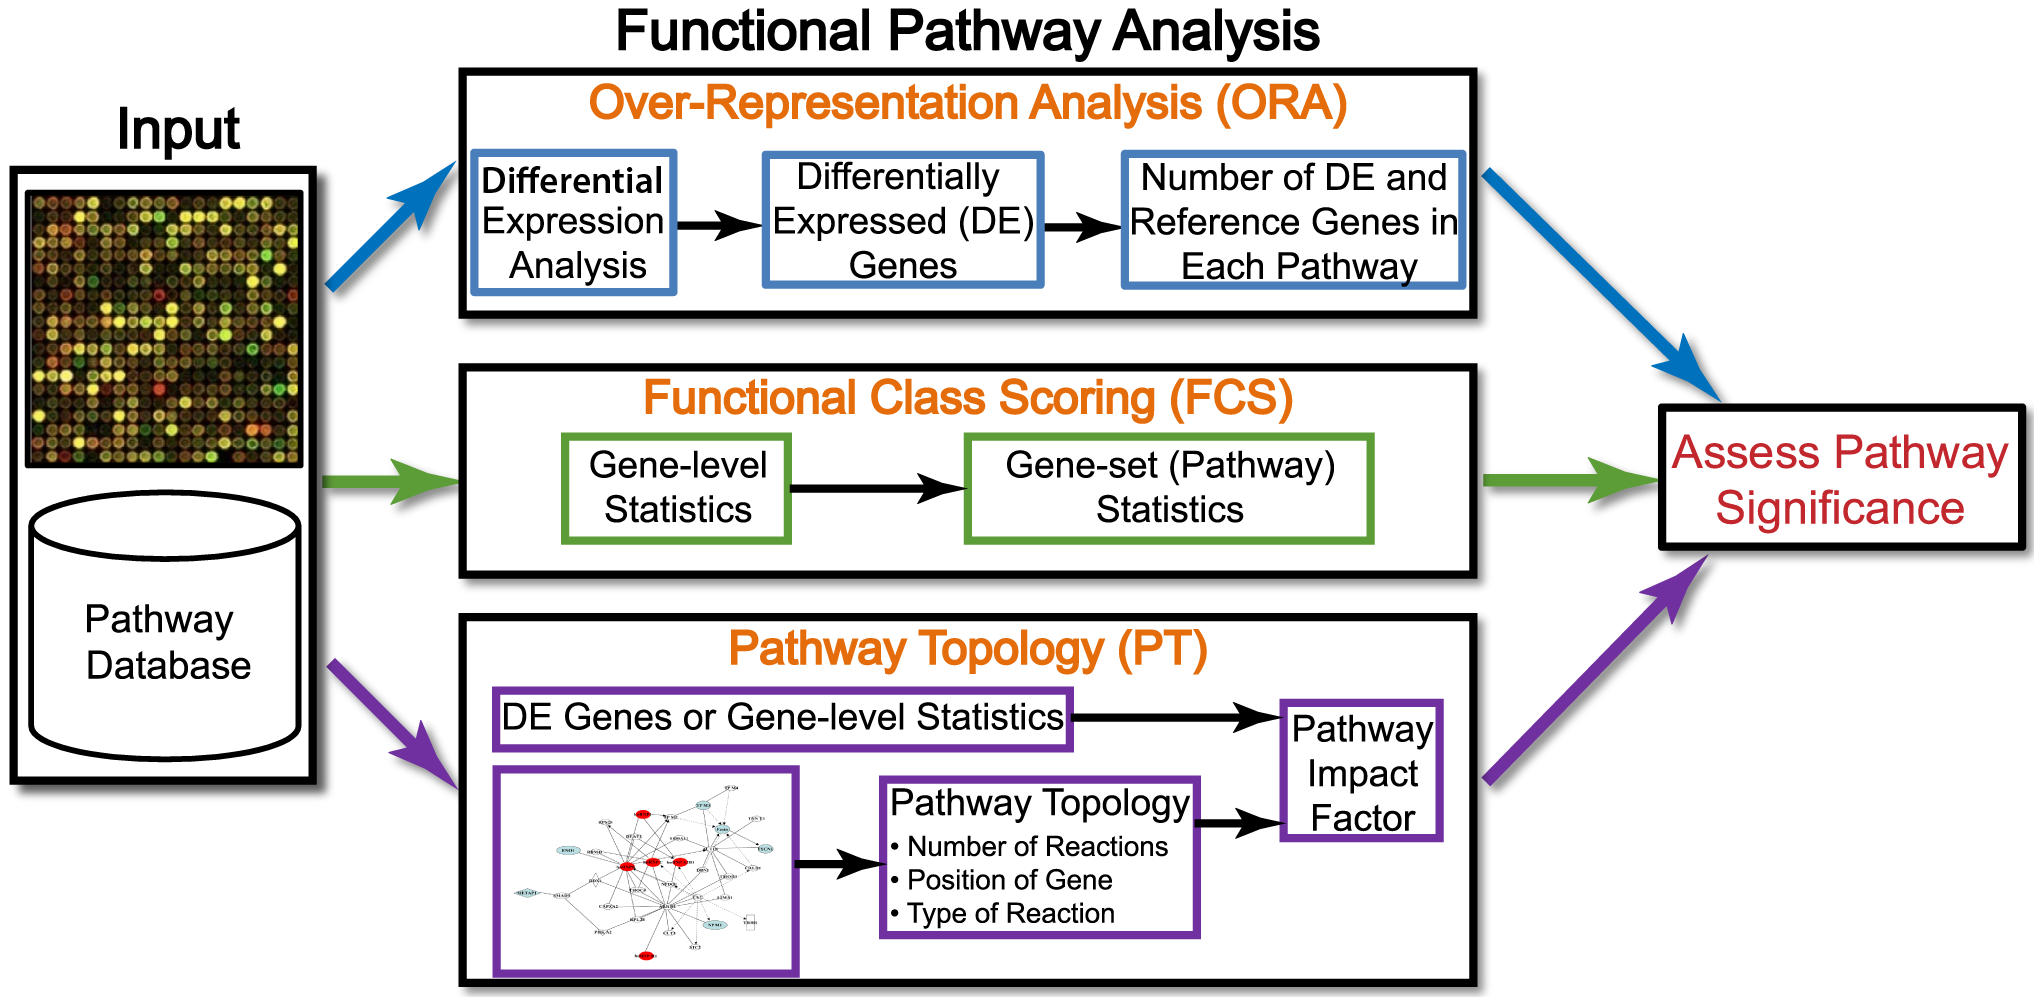
\includegraphics[width=0.9\textwidth]{Pipeline_Pathway.png} 
\caption{El procès d'anàlisi de les rutes}
\end{figure}



\subsection{ORA}

L'anàlisi de sobreexpressió és una tècnica d'identificació de les rutes significativament enriquides en la mostra d'interès. 

El paper original que se cita habitualment quan es parla d'anàlisi d'expressió genètica és de \cite{boyle2004go}. El mètode estadístic descrit consisteix bàsicament en els passos següents:

\begin{enumerate}
\item \textbf{De tots els gens de la mostra seleccionar un grup de gens que es considera que són significativament expressats.}

Els criteris de selecció poden basar-se en \textit{log ratios} i/o en el valor de p provinent d'un test estadístic. \textit{Log ratios} donen la magnitud amb la qual un gen és sobre o sotaexpressat. Les diferències entre els grups però són el resultat d'un procès estochàstic i per tant hem d'intentar de minimitzar el risc de prendre decisions falses. El valor de p representa la probabilitat d'aquest risc i per tant dona certa confiança sobre la significació de les diferències observades.

\item \textbf{Determinar si algunes rutes anoten la llista especificada de gens amb la freqüència més alta que la que s’esperaria per casualitat.} 

El test estadístic es basa en la distribució hipergeomètrica: 

$$p = 1 - \displaystyle\sum_{i = 0}^{k-1}\frac{{M \choose i}{{N-M} \choose {n-i}}} {{N \choose n}}$$

En aquesta equació $N$ és el nombre total de gens en la distribució de fons, $M$ és el nombre de gens dins d'aquesta distribució que són anotats a la ruta d'interès, $n$ és el nombre total en la llista especificada de gens i $k$ és el nombre de gens dins d'aquesta llista que són anotats a la ruta. La distribució de fons pot ser o bé tots els gens en la base de dades d'anotació o bé tots els gens de l'experiment.

El valor de P obtingut amb aquesta fòrmula dona la probabilitat de veure el nombre $x$ de gens de la llista relacionats amb la ruta específica en la llista del nombre total de gens $n$ donat la proporció de gens relacionats amb aquesta ruta en la distibucó de fons.
\end{enumerate}

L'aplicació utilitza aquesta idea i calcula una taula amb els camps següents:


\begin{itemize}
\item \underline{Description}. El nom del terme GO;
\item \underline{GeneRatio}. El quocient: $\displaystyle\frac{\mbox{Nombre dels gens diferencialment expressats que pertanyen al conjunt de gens}}{\mbox{Nombre total dels gens diferencialment expressats}}=\frac{M}{N}$; 
\item \underline{BgRatio}. El quocient: $\displaystyle\frac{\mbox{Nombre dels gens del conjunt d'interès en la distribució de fons}}{\mbox{Nombre total dels gens en la distribució de fons}}=\frac{k}{n}$;
\item \underline{pvalue}. Valor de p basat en la distribució hipergeomètrica descrita anteriorment.
\item \underline{p.adjust}. El valor de P ajustat. L'usuari pot seleccionar el mètode d'ajustmanent.
\end{itemize}


\subsection{GSEA}

Amb l'anàlisi GSEA podem analitzar els resultats d'un experiment d'expressió per a dos grups. Aquí els gens són ordenats basant-se en la correlació entre la seva expressió i la separació entre les classes. Aquest llistat ordenat $L$ el podem crear utilitzant els \textit{logRatios}.

Donat el conjunt definit dels gens $S$, que pertanyen per exemple al mateix terme de Gene Ontology, l'objectiu de GSEA és determinar si els membres de $S$ són distribuïts aleatòriament en el $L$ o es troben més al cap o a la cua. S'esperaria que els gens relacionats amb la separació fenotípica mostraran aquesta última distribució. 

L'anàlisi GSEA consisteix en tres passos:

\begin{enumerate}
\item Càlcul de la puntuació d'enriquement (\textit{ES: Enrichment Score}). La puntuació està calculada anant per la llista i augmentant la suma corrent sempre quan es troba un gen que pertany a $S$ o, al contrari, restant-la quan el gen no forma part del conjunt $S$. La puntuació és la desviació màxima del zero observada en aquet camí. L'estadística obtinguda és l’estadística de Kolmogorov-Smirnov amb pesos.

\item Estimació del nivell de significació per a la puntuació \textit{ES}. El valor de P nominal es pot obtenir mitjançant o bé la permutació de les classes o bé la permutació de gens, on l'estadística \textit{ES} observada es compara amb la distribució obtinguda amb permutació. A l'aplicació es fa ús de l'útima opció.
\item Càlcul del valor de P ajustat. El valor de P nominal s'ajusta per controlar l'error global que es produeix com a resultat de les comparacions múltiples.
\end{enumerate}

\begin{figure}[H]
\centering
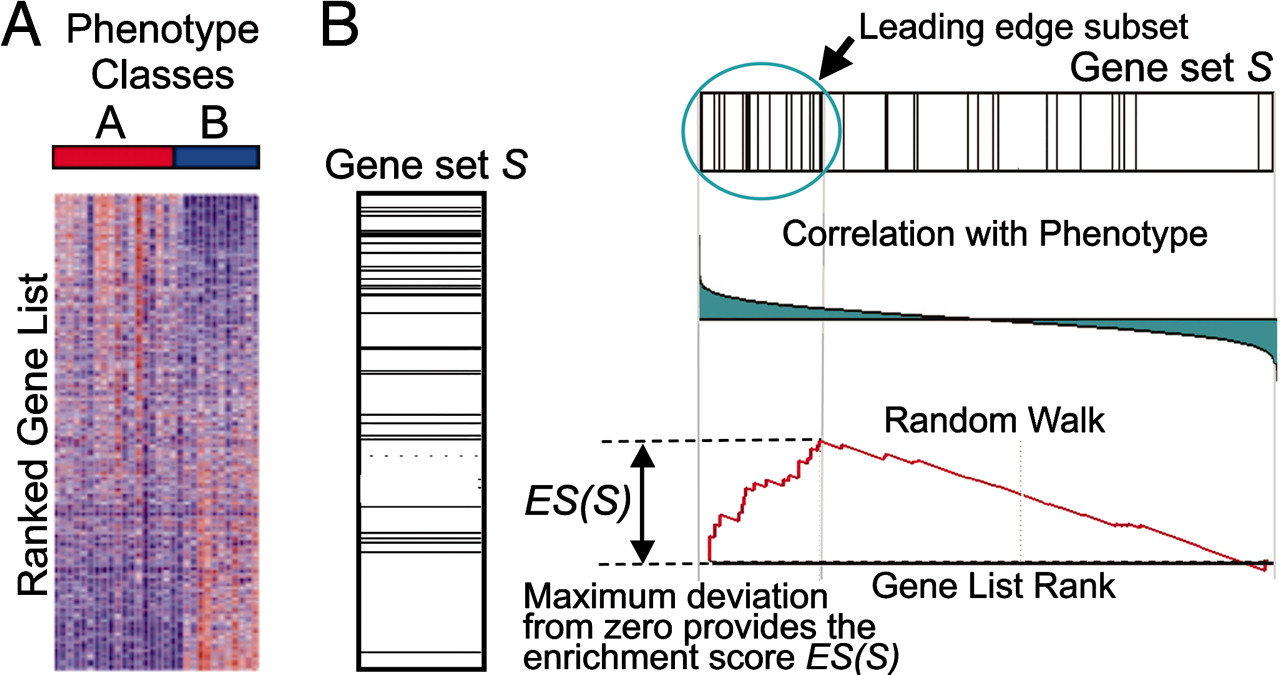
\includegraphics[width=0.9\textwidth]{GSEA_Method.jpg} 
\caption{El mètode GSEA}
\end{figure}

L'aplicació que he desenvolupat agafa aquesta idea i calcula la taula que inclou les estadístiques següents:

\begin{itemize}
\item \underline{enrichmentScore}. Enrichment score per al conjunt dels gens. Amb altres paraules: el grau amb el qual el conjunt dels gens està sobreexpressat a dalt o a baix del llistat ordenat dels gens en les dades d'expressió.
\item \underline{NES}. Normalized enrichment score. La puntuació per al conjunt de gens després de ser normalitzat tenint en compte tots els conjunts de gens analitzats (la seva mida i la seva correlació amb les dades d'expressió). Aquesta puntuació ajuda a comparar els resultats entre els conjunts de gens.
\item \underline{pvalue}.El valor de p nominal.
\item \underline{p.adjust}. El valor de p ajustat.
\item \underline{leading\_edge}
\begin{itemize}
\item \underline{Tags}. El percentatge de les ocurrències de gens del conjunt específic abans (per als ES positius) o després (per als ES negatius) del cim en la puntuació corrent d'enriquiment. Aquest valor indica el percentatge dels gens que contribueixen a la puntuació d'enriquement. 
\item \underline{List}. El percentatge dels gens en el llistat ordenat de tots els gens abans o després del pic en la puntuació corrent d'enriquiment. Aquest valor ens indica on exactament el pic es produeix. 
\item \underline{Signal}. La fortalesa del senyal d'enriquiment que combina els dos valors anteriors.
\end{itemize}
\item \underline{rank}. La posició del pic en la llista ordenada dels gens. Els conjunts dels gens més interessants assoleixen el seu màxim o bé al principi o al final de la llista ordenada. Vol dir que tenen aquest valor o bé molt baix o bé molt alt.
\end{itemize}

\subsection{L'anàlisi topològic de les rutes}
Tan ORA com GSEA no visualitzen les relacions entre les rutes i entre els gens dins de les rutes. Els avenços en anotació manual de les bases de dades disponibles (GO, KEGG i Reactome) contenen però aquesta informació i l'aplicació, gràcies al paquet \helvetica{clusterProfiler}, hi treu l'avantatge i visualitza aquestes relacions més detalladament. 

\subsubsection{El mapa d'enriquement}

Navegant a la categoria \textbf{Enrichment plot} l'usuari obté el mapa d'enriqument. El mapa organitza les rutes en una xarxa amb les línies que connecten les rutes amb els gens solpats. D'aquesta manera les rutes amb gens en comú s'agrupen més a prop l'una de l'altra.

\subsubsection{Gene-Concept-Network}

L'anàlisi ORA no visualitza per si sola els gens que contribueixen al fet que la ruta sigui diferencialment expressada. Amb la xarxa de gens-concepte es pretén visualitzar els gens al voltant dels conceptes on els gens poden ser connectats amb les rutes (conceptes) diferents. D'aquesta manera es fa possible identificar les associasions biològiques més complexes entre les rutes mitjançant els gens. 

\subsubsection{GOplot}
%Per a mès informació http://geneontology.org/docs/ontology-relations/

El gràfic de GO està organitzat com direccional acíclic gràfic (Directed Acyclic Graph). Una manera útil de veure els resultats és mirar com els termes GO estan distribuïts per aquest gràfic. L'aplicació ensenya el gràfic GO induït pels els gens més significatius. El gràfic mostra tres relacions possibles entre les rutes: 
\begin{enumerate}
\item \textit{is a}: Si dèiem que A \textit{is a} B, volem dir que A és un subtip de B. Per exemple el cicle mitòtic de la cèl·lula \textit{is a} cicle de la cèl·lula. 
\item \textit{part of}: Aquesta relació s'utilitza per representar la relació entre una part i el tot. Aquesta relació entre A i B existeix nomès si B és necessàriament una part d'A: quan B existeix, ho fa només com una part de B i la presència de B implica la presència d’A.
\item \textit{regulates}: La relació descriu el cas on un procès afecta directament la manifestació de l'altre procès.
\end{enumerate}

Els conceptes al llarg del gràfic són marcats amb color depenent si són estadísticament significatius o no.

\subsubsection{KEGG Pathway}
%Per a més informació sobre l'anotació https://www.genome.jp/kegg/document/help_pathway.html
Aquest gràfic mostra les relacións entre els gens dins de la ruta específica. Els gens són remarcats amb el color depenent de l'expressió diferencial mesurada amb LogRatios. Per poder interpretar el gràfic és útil tenir present l'anotació següent:

\begin{figure}[H]
\centering
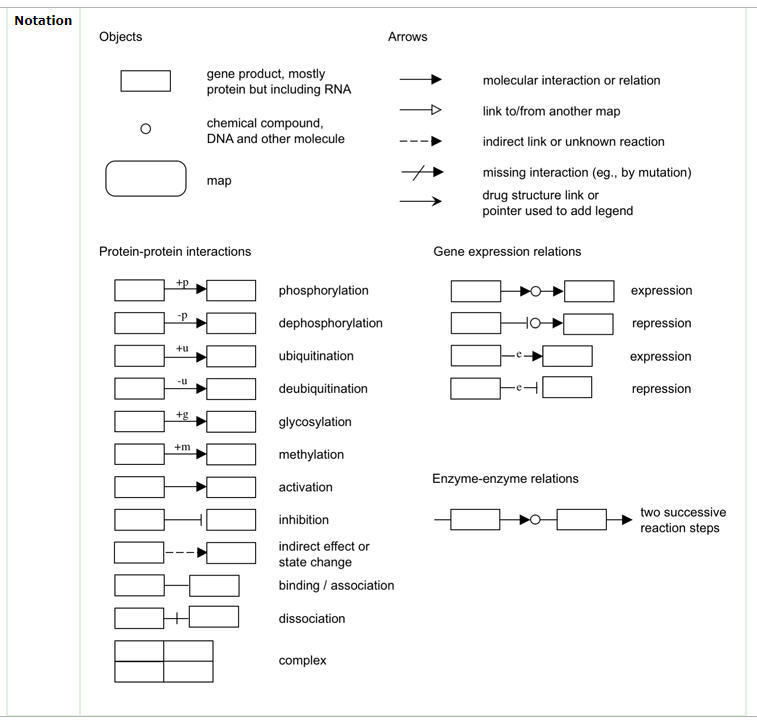
\includegraphics[width=0.9\textwidth]{Annotation_KEGG.jpg} 
\caption{L'anotació de les relacions dins de les rutes KEGG}
\end{figure}

\subsubsection{Reactome Pathway}
En canvi a Goplot i les rutes KEGG les relacions entre els gens dins les rutes Reactome són més senzilles. Aquí les relacions són mostrades només amb les línies, on es pot interpretar només la distància entre els gens. 



\section{Instal·lació de l'aplicació}

La solució més plausible i ràpida era empaquetar tota l'aplicació dins d'un paquet R i fer-la disponible d'aquesta manera en el GitHub. Hi havia també dues opcións més: 

\begin{itemize}
\item Publicar l'aplicació a CRAN
\item Publicar l'aplicació en un servidor Shiny
\end{itemize}
La primera opció, publicació en CRAN, no l’he contemplat encara, perquè la solució no és immediata, sino que és un procès que no és fàcil i pot tardar fins que el paquet estigui
 publicat amb éxit. Com comenta \cite{HWick} \enquote{submitting to CRAN is a lot more work than just providing a version on github, but the vast majority of R users do not install packages from github, because CRAN provides discoverability, ease of installation and a stamp of authenticity. The CRAN submission process can be frustrating, but it’s worthwhile...}. Normalment els paquets han d’estar en perfectes condicions abans d'entregar-los i seran revisats manualmet per un equip dels voluntaris. D'aquesta manera l'aplicació no seria avaluable dins del marc temporal previst per al treball de màster. A més a més considero que podria millorar encara més l'aplicació abans d'entregar-lo.

La segona opció, publicació via Shiny Server, és molt interessant, però implicaria un treball considerable per configurar el servidor. Com que ho faria per primera vegada, no puc assegurar que tot estigui preparat a temps. 

Per tant, el paquet \helvetica{PathwayApp} es pot instal•lar del repositori GitHub seguint els passos següents:

\begin{enumerate}
\item Instal·lar, si encara no està fet, la versió actual de R;

\item Instal·lar, si encara no està fet, el Bioconductor;

\item Instal·lar, si encara no està fet, el paquet \helvetica{devtools}

\begin{lstlisting}[language=R]
install.packages(``devtools'')
library(devtools)
\end{lstlisting}

\item Instal·lar el paquet \helvetica{PathwayApp}

\begin{lstlisting}[language=R]
devtools::install_github("vdruchkiv/TFM/5_Packages/PathwayApp/PathwayApp")
\end{lstlisting}

\item Iniciar l'aplicació 
\begin{lstlisting}[language=R]
PathwayApp::runPathwayApp()
\end{lstlisting}
\end{enumerate}

La funció \helvetica{runPathwayApp()} iniciarà la comprovació dels paquets necessaris i començarà l'aplicació. Els paquets següents seran instal·lats, si no ho són encara:

\begin{center}
\begin{tabular}{||c | c ||} 
\hline\hline 
\textbf{Paquet} & \textbf{Font} \\ [0.5ex] 
\hline\hline
clusterProfiler & Bioconductor \\
\hline
ReactomePA & Bioconductor \\
\hline
pathview & Bioconductor \\ 
\hline
pathviewPatched & GitHub vdruchkiv/TFM\\
\hline
dplyr & CRAN \\
\hline 
ggplot2 & CRAN \\
\hline
knitr & CRAN \\
\hline
kableExtra & CRAN \\
\hline
formattable & CRAN \\
\hline
shiny & CRAN \\
\hline 
shinydashboard & CRAN \\ 
\hline
shinyhelper & CRAN \\
\hline 
shinycssloaders & CRAN\\
\hline\hline
\end{tabular}
\end{center}



\section*{Biblilografia}
\addcontentsline{toc}{section}{Biblilografia}
\renewcommand{\section}[2]{}%
%\renewcommand{\chapter}[2]{}% for other classes
\bibliography{references}
\bibliographystyle{apalike}


\end{document}



